\documentclass[a4paper]{scrartcl}

% Font and Language
\usepackage[utf8]{inputenc}
\usepackage[T1]{fontenc}
\usepackage[english]{babel}
\usepackage{lmodern}

% Do not change font size, parskip or margin.
%Attempts to make a shorter paper appear larger will lead to course failure.
\KOMAoptions{fontsize=12pt}
\KOMAoptions{parskip=off}

\usepackage[
	left=2.5cm,
	right=2.5cm,
	top=2.5cm,
	bottom=4.5cm
]{geometry}

% Bibliography
\usepackage[backend=biber]{biblatex}
\usepackage{csquotes}
\addbibresource{references.bib}

% Add blindtext
\usepackage{blindtext}

% Running heads and foots
\usepackage[headsepline,footsepline]{scrlayer-scrpage}

% Set title

\newcommand{\paperTitle}{ComfortSphere: A Smart Home System for\\ Indoor Environment Optimization}
\title{\paperTitle}
\clearpairofpagestyles
\rehead{\paperTitle}
\rohead{\paperTitle}

% Set your name, your mail and matrikel number
\newcommand{\paperAuthor}{Joshi Juhi Ramesh, Amardeep Mishra,\\ Hardikkumar Savaliya, Mohammad Sheikh,\\ Riya varghese, Hammad Chaudhary}
\author{
    Juhi Joshi~<jr.joshi@stud.fh-sm.de>, 316800\\
    Amardeep Mishra~<a.mishra@stud.fh-sm.de>, 316652\\
    Hardikkumar Savaliya~<hv.savaliya@stud.fh-sm.de>, 313904\\
    Mohammad Sheikh~<mzi.sheikh@stud.fh-sm.de>, 312538\\
    Hammad Chaudhary<rehman@stud.fh-sm.de>, 313955\\
    Riya varghese~<rm.varghese.a@stud.fh-sm.de>, 316773
    }

\lehead{\paperAuthor}
\lohead{\paperAuthor}




% Set page numbering
\usepackage{lastpage}
\refoot{\thepage{}of\pageref{LastPage}}
\rofoot{\thepage{}of\pageref{LastPage}}

% Add suas logo
\usepackage{graphicx}
\KOMAoptions{footheight=3cm}
\lefoot{\vspace*{1.5in}
\includegraphics[height=1cm]{suas-logo}}
\lofoot{
\includegraphics[height=2cm]{suas-logo}}

% Do not show date
\date{}

\begin{document}
	\maketitle

\section{Introduction}
The field of IoT-enabled smart home systems has experienced exponential growth, with applications ranging from simple remote controls to complex, automated home ecosystems. ComfortSphere proposes an advanced smart room ecosystem tailored for optimal indoor climate control, leveraging precise sensor data and automated adjustments. This system is designed to address the specific needs of health-conscious individuals and those with respiratory issues.

\subsection{Use Case}
ComfortSphere is tailored for users requiring real-time monitoring of temperature and humidity, particularly in settings where fluctuating indoor conditions adversely impact health. For instance, individuals with asthma or COPD benefit from consistent humidity levels; ComfortSphere maintains this by dynamically adjusting indoor climate based on sensor readings and user preferences.

\subsection{Broader Relevance}
Automated climate control not only promotes individual well-being but also provides energy savings and security, impacting personal health and broader goals of sustainable energy consumption. ComfortSphere is designed for a wide range of users, from homeowners to healthcare and security engineers, with applications in both residential and healthcare facilities.

\subsection{Scope}
This research integrates and optimizes smart sensors (DHT22, light and motion sensors), microcontroller programming (using Pinecone), and app-based remote access to manage and monitor indoor climate parameters effectively.

\section{Literature Review}
This section reviews current research on smart home automation, sensor-based environmental monitoring, health impacts of indoor air quality (IAQ), and energy-efficient automation.

\subsection{Humidity-Based Temperature Control Using IoT}
The study [1] “Humidity Based Automated Room Temperature Controller Using IoT” demonstrates a humidity-based automated temperature control system with an electric heater for precise climate regulation. However, it lacks integration of health-specific metrics or energy-efficient features, which ComfortSphere addresses.

\subsection{Energy Efficiency in Smart Buildings through IoT Approaches}
This study by[2] Metallidou, Psannis, and Egyptiadou focuses on energy-efficient automation in smart buildings using IoT technologies. The authors describe how low-cost IAQ sensors can enable smart ventilation controls, allowing systems to operate based on pollutant levels instead of on fixed schedules. By incorporating real-time air quality data, these systems can maintain indoor air quality while conserving energy by only ventilating as needed.\\

Implications:
The research demonstrates that integrating cost-effective sensors into smart building systems offers a balance between energy savings and maintaining a safe indoor environment. The approach described here is particularly useful in energy-sensitive spaces, as it prevents overuse of HVAC systems. This contributes to lower operational costs and less environmental impact by activating ventilation or air purification only when pollutant levels rise above safe limits. Such systems support a sustainable approach to indoor environment management, maximizing health protection while minimizing energy consumption.

\subsection{A Review of IoT Applications in Smart Home Automation}
The study[3] Sepasgozar, Karimi, Farahzadi, and Moezzi provide an extensive review of IoT and AI applications in smart home automation, exploring systems such as smart air control, solar energy integration, and environmental monitoring. They discuss technologies that improve both energy efficiency and indoor air quality. One area of focus is how these systems integrate solar energy to power climate control, thus enabling more eco-friendly and cost-effective ventilation and air quality management.\\

Implications:
The study underscores the potential for integrating renewable energy sources with IoT-driven environmental sensors to enhance sustainability in home automation. By combining solar power with air quality monitoring and ventilation control, these systems reduce energy costs and environmental impact. The findings suggest that hybrid systems can create healthier living spaces while promoting sustainable energy use, making them a compelling option for modern households.

\subsection{Portable Humidity and Temperature Monitoring Nodes}
The portable node described in [4] ”A portable node of humidity and temperature sensor for indoor environment monitoring” is a compact, cost-effective system designed for smart home monitoring, featuring a DHT11 sensor, Zigbee module, STM32L100 microcontroller, and a smartphone interface. Its portability and low-power consumption make it convenient for indoor monitoring. However, the system’s capabilities are limited to basic data collection and do not extend to automated climate adjustments or health-specific features. ComfortSphere advances this concept by integrating a DHT22 sensor with higher precision and incorporating motion-sensing for adaptive, energy-efficient automation, allowing it to serve not only as a monitoring tool but as a health-oriented, automated climate control system.

\subsection{Intelligent Indoor Temperature and Humidity Control}
The indoor climate control system designed in [5]“Intelligent Indoor Temperature and Humidity Control System” aims to overcome the limitations of traditional climate control by using wireless communication and control algorithms, adjusting settings to maintain ideal temperature and humidity levels. The use of wireless modules and real-time monitoring enables the system to control HVAC components like air conditioners and humidifiers, enhancing user comfort. While this system is effective in maintaining a stable indoor environment, it lacks real-time, health-specific calibrations and personalized climate adjustments. ComfortSphere fills this gap by dynamically optimizing IAQ based on user-defined health needs, offering personalized adjustments for individuals with asthma or COPD.

\subsection{Intelligent Monitoring for Indoor Environments System}
In [6]“Indoor Environment Intelligent Monitoring System”, the development of an indoor environmental monitoring system leverages an STM32 microcontroller and SHT10 sensor to track indoor temperature and humidity data. Users can remotely access real-time and historical data, enabling them to observe trends and system performance. Although long-term testing confirms the system’s stability and accuracy, it primarily functions as a monitoring solution without active climate control capabilities. ComfortSphere extends this approach by not only monitoring but actively adjusting indoor conditions to improve IAQ for health-conscious users, integrating motion-based automation for added energy efficiency.

\subsection{ Health Impacts of Humidity on Respiratory Well-Being}
Research by [7] “Effects of Low Humidity and High Humidity on the Nasal Area of the People” investigates how varying humidity levels influence respiratory health, particularly through symptoms like nasal congestion, dryness, and sneezing. Findings show that exposure to low humidity can lead to nasal and skin dryness, while high humidity increases congestion. This study highlights the need for systems that maintain a balanced indoor climate, which is essential for individuals with respiratory sensitivities. ComfortSphere aligns with these findings by maintaining optimal humidity levels (40-60%) to prevent health issues associated with poor IAQ, based on WHO recommendations, making it a health-supportive alternative to standard smart thermostats.
By addressing limitations in each of these studies, ComfortSphere contributes to the evolving field of IoT-enabled smart home systems, focusing on adaptive climate control to promote respiratory health, user-centric customization, and energy-efficient automation.

\subsection{Optimizing Energy-Efficient Automation with Thermal Control}
[8] Erişen’s study delves into energy-efficient automation that manages thermal comfort in smart buildings. The focus is on predictive algorithms that assess indoor temperature needs while also considering IAQ. By factoring in pollutant levels alongside temperature, these models allow smart systems to balance air quality and thermal comfort, automatically making adjustments that reduce heating and cooling costs while preventing the buildup of indoor pollutants.\\

Implications:
The predictive approach described in this paper enables smart systems to learn from climate data to maintain optimal indoor conditions. Erişen’s model supports energy efficiency by ensuring that heating or cooling is applied only when necessary, preventing energy wastage. This study suggests that combining air quality and thermal control leads to more effective IAQ management, reducing health risks associated with indoor pollutants while optimizing energy use.

\subsection{Smart Light Using PIR Sensor}
The study [9] “Smart Light Using PIR Sensor” aligns with the adaptive lighting goals of ComfortSphere by employing motion detection to conserve energy and enhance user convenience. It proposes efficient, scalable, and cost-effective lighting solutions that can be seamlessly integrated into broader smart home systems like ComfortSphere. Unlike standalone lighting systems, ComfortSphere combines PIR-based adaptive lighting with other health and energy-efficient features, offering a holistic approach to smart home automation.\\



% Continue with each sub-section for Literature Review as per the content in the provided proposal

\section{Research Question}
The primary research question is:

\begin{itemize}
    \item How effectively can ComfortSphere manage and optimize indoor environmental conditions to support health and energy efficiency in a smart home setting?
    \item How accurately does the DHT22 sensor maintain optimal temperature and humidity levels in real-time?
    \item What measurable impact does automated climate control, based on occupancy data, have on energy savings?
    \item To what extent does motion-sensor integration enhance safety and convenience?
    \item How does the ComfortSphere app improve user engagement with environment monitoring?
    \item How can IoT technology improve the real-time monitoring and regulation of indoor conditions specifically temperature and humidity?
\end{itemize}
\section{Methodological Design}
\begin{figure}[th]
    \centering
    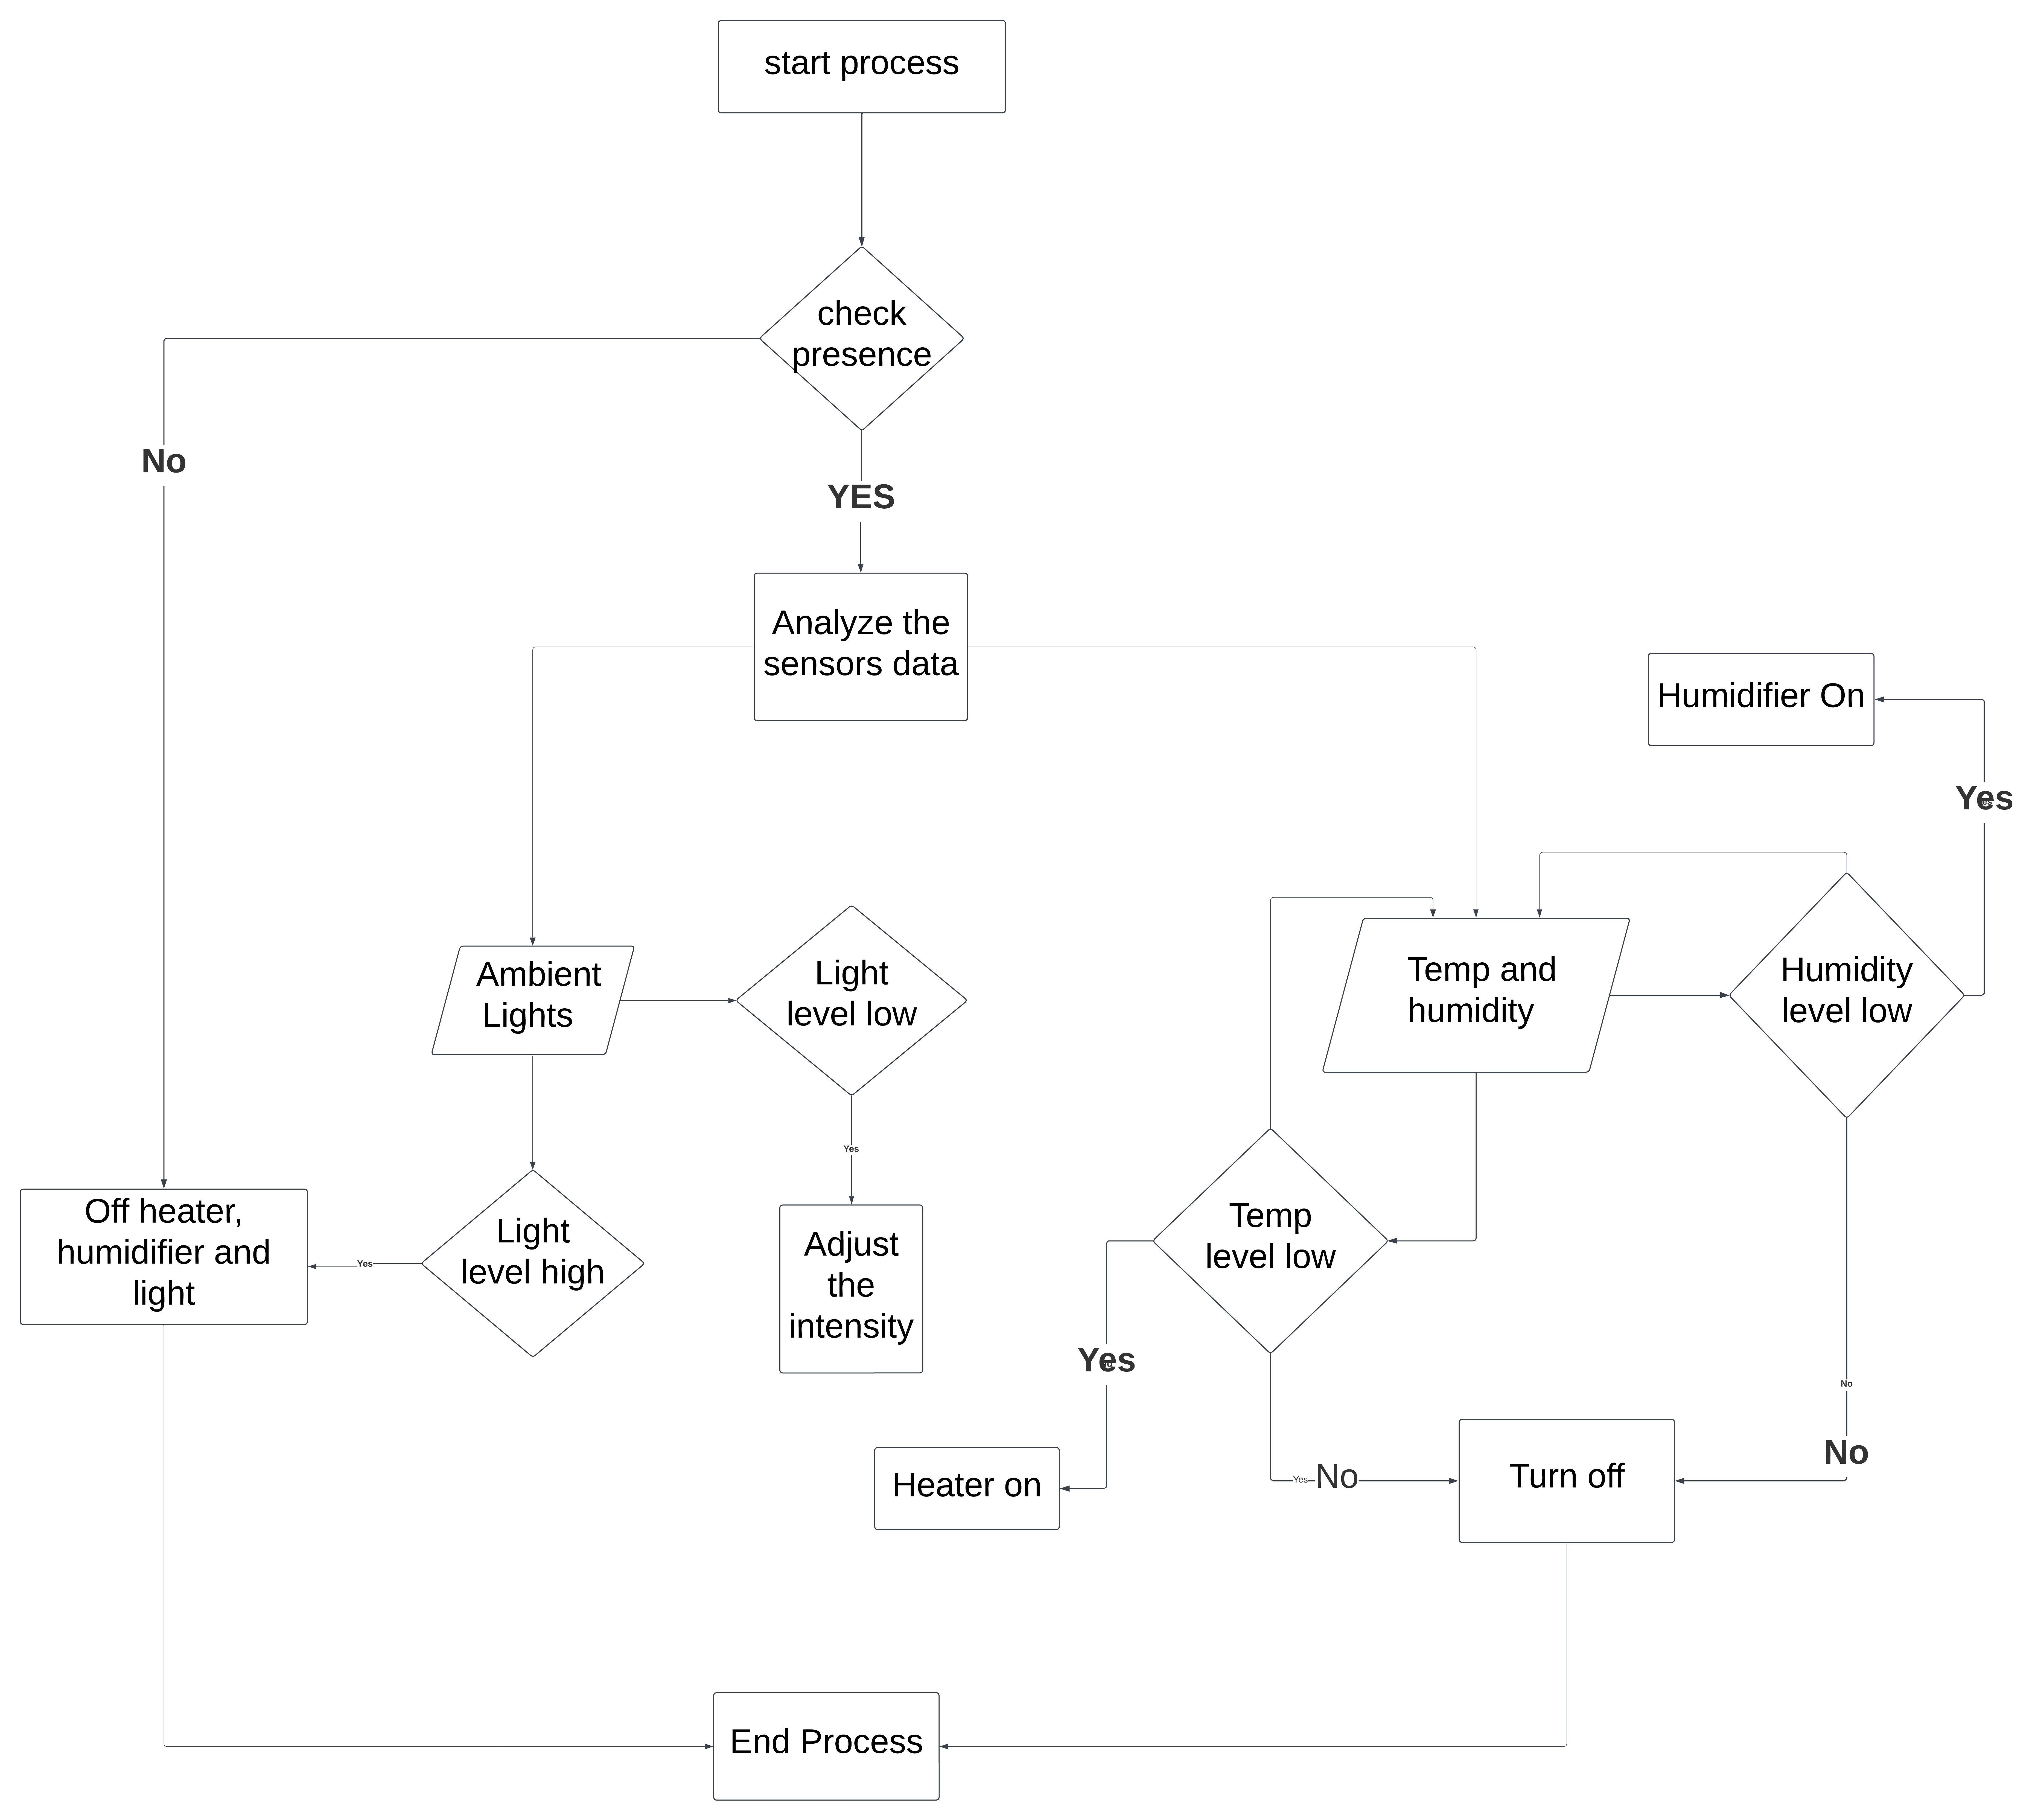
\includegraphics[width=\linewidth]{diagram.jpg.png}
    \caption{Flowchart of the system}
    \label{fig:my_label}
\end{figure}
The methodological design includes experimental setup, data processing, and user interaction with the ComfortSphere system.
\subsection{Approach}
A quantitative experimental approach will test system accuracy, response time, and energy efficiency, with qualitative feedback on usability and health benefits.

\begin{figure}[th]
    \centering
    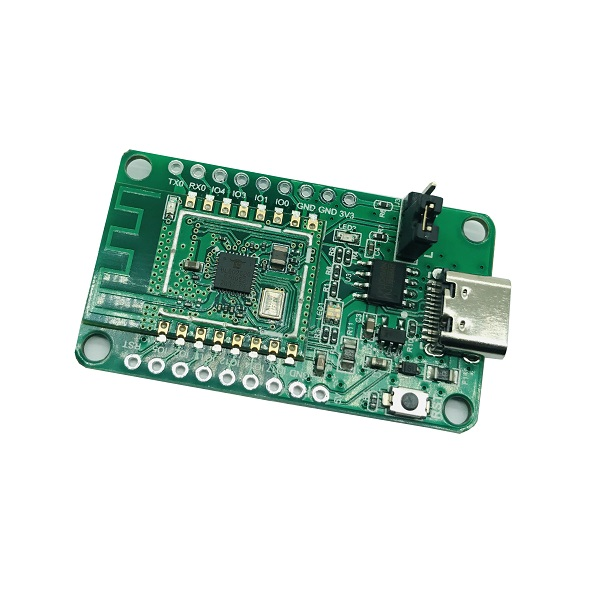
\includegraphics[width=0.5\textwidth]{Pinecone-1.jpg}
    \caption{Pinecone-microcontroller}
    \label{fig:my_label}
\end{figure}
\newpage

\subsection{Data Collection and Access}
\textbf{Sensors:} Data will be collected using the DHT22 (for temperature
and humidity), an occupancy-detecting motion sensor. and a light
sensor for ambient lightning. Sensor readings will be continuously
logged via the Pinecone microcontroller, and then transmitted to the
ComfortSphere app.

\textbf{User Interaction:} Users will interact with the app to set climate preferences, toggle lights, monitor real-time data, and review historical
records. User feedback will be collected through surveys and structured interviews to assess satisfaction and health impacts.


\subsection{Use Cases and Experiment Selection}
Three user profiles will be studied:
\begin{enumerate}
    \item Health-focused: Users with asthma or respiratory concerns.
    \item Energy-conscious: Users focused on cost and energy efficiency.
    \item Safety-conscious: Elderly or vulnerable individuals for whom safety features are essential.
\end{enumerate}
Each group will use the system for two weeks, followed by an analysis of performance, energy usage, and satisfaction.

\subsection{Time Frame}
The experimental phase will last approximately two months, with additional time allocated for data analysis, system calibration, and refinement.

\subsection{Data Recording and Processing}

\begin{itemize}
    \item \textbf{Data Recording:} Sensor data will be recorded on the Pinecone microcontroller and uploaded to a cloud server, accessible via the ComfortSphere app.
\end{itemize}

\begin{itemize}
    \item \textbf{Data Analysis:} Quantitative data on temperature, humidity, and
energy consumption will be processed using statistical software to analyze trends, variance, and correlation with user preferences and occupancy.
\end{itemize}

\begin{itemize}
    \item \textbf{User Feedback:} Survey responses will be analyzed with thematic coding to identify patterns in satisfaction and health-related responses.
\end{itemize}

\subsection{Presentation of Findings}
Results will be presented in graphical formats (e.g., line and bar charts), with statistical analyses illustrating correlations between environmental parameters and health outcomes.

\section{References}
\begin{enumerate}
    \item Farah Sharmin et al. “Humidity Based Automated Room Temperature Controller Using
IoT”. In: 2019 Third International conference on I-SMAC (IoT in Social, Mobile,
Analytics and Cloud) (I-SMAC). 2019, pp. 226–231. doi: 10.1109/I-SMAC47947.
2019.9032624.
    \item C. K. Metallidou, K. E. Psannis and E. A. Egyptiadou, "Energy Efficiency in Smart Buildings: IoT Approaches," in IEEE Access, vol. 8, pp. 63679-63699, 2020, doi: 10.1109/ACCESS.2020.2984461.
keywords: {Europe;Sensors;Smart cities;Smart buildings;Monitoring;Phase change materials;Energy efficiency;energy performance of existing buildings;Internet of Things;smart building template;smart energy management},

    \item Sepasgozar, S.; Karimi, R.; Farahzadi, L.; Moezzi, F.; Shirowzhan, S.; M. Ebrahimzadeh, S.; Hui, F.; Aye, L. A Systematic Content Review of Artificial Intelligence and the Internet of Things Applications in Smart Home. Appl. Sci. 2020, 10, 3074. https://doi.org/10.3390/app10093074
    
    \item Trio Adiono et al. “A portable node of humidity and temperature sensor for indoor
environment monitoring”. In: 2018 3rd International Conference on Intelligent Green
Building and Smart Grid (IGBSG). 2018, pp. 1–5. doi: 10 . 1109 / IGBSG . 2018 .
8393575.
    \item Shuo Sun and Yukun Ma. “Intelligent Indoor Temperature and Humidity Control System”.
In: 2022 2nd International Conference on Electronic Information Engineering
and Computer Technology (EIECT). 2022, pp. 28–33. doi: 10.1109/EIECT58010.
2022.00011.

    \item Jiaqiang Li et al. “Indoor Environment Intelligent Monitoring System”. In: 2018
IEEE International Conference on Mechatronics and Automation (ICMA). 2018,
pp. 1446–1451. doi: 10.1109/ICMA.2018.8484267.

    \item Kenneth Vance R. Arcenal, Matthim S. Carmen, and Ramon G. Garcia. “Effects of
Low Humidity and High Humidity on the Nasal Area of the People”. In: 2023 IEEE
IAS Global Conference on Emerging Technologies (GlobConET). 2023, pp. 1–6. doi:
10.1109/GlobConET56651.2023.10149971.

    \item Erişen, S. A Systematic Approach to Optimizing Energy-Efficient Automated Systems with Learning Models for Thermal Comfort Control in Indoor Spaces. Buildings 2023, 13, 1824. https://doi.org/10.3390/buildings13071824
    
    \item Subashini, Dharrsan, V., Immanuel, C., and Deepak. (2018). Smart light using PIR sensor [Journal-article]. International Journal for Research Trends and Innovation, 3(10), 225. https://www.ijrti.org/papers/IJRTI1810038.pdf
    
    % Add additional references as needed
\end{enumerate}
\end{document}